\documentclass[12pt,a4paper,pagesize=pdftex]{scrartcl}
\usepackage[latin1]{inputenc}
\usepackage[english]{babel}
\usepackage{amsmath}
\usepackage{amsthm}
\usepackage{amssymb}
\usepackage{lmodern}
\usepackage{color}
\usepackage{graphicx}
\usepackage{caption}
\usepackage{textcomp}
\usepackage{gensymb}
\usepackage{listings}
\usepackage{algorithm}
\usepackage{algorithmic}
\usepackage{algorithmic}
\usepackage{units}
\usepackage{hyperref}
\usepackage{float}
\usepackage{mathtools}
\lstset{frame = single, breaklines=true, postbreak=\raisebox{0ex}[0ex][0ex]
{\ensuremath{\color{red}\hookrightarrow\space}}}
\usepackage[pass,letterpaper]{geometry}
\usepackage[section]{placeins}
\graphicspath{ {.} }
\renewcommand{\thesubsection}{\thesection\alph{subsection}}
\newcommand{\comment}[1]{}
\title{Numerical Solution and Implementation of the Jointly Markovian Probability Master Equations}
\subtitle{}
\author{}
\date{}
\linespread{1.25}

\begin{document}

\pdfpageheight 11in
\pdfpagewidth 8.5in

\maketitle

% BEGIN DOCUMENT
\section*{Probability Master Equations}
The probability master equations start as a coupled system of two equations with non-constant coefficients dependent on the \(\phi\) and \(\theta\) domains:

\begin{multline*}
    \frac{\partial}{\partial t} \left(p_1 P_1 \left(\phi, \theta, t\right)\right) + \frac{\partial}{\partial \phi} \left(f_1\left(\phi, \theta\right) p_1 P_1 \left(\phi, \theta, t\right)\right) + \frac{\partial}{\partial \theta} \left(g_1 \left(\phi, \theta\right) p_1 P_1\left(\phi, \theta, t\right)\right) \\= \frac{p_2}{\tau_2} P_2 \left(\phi, \theta, t\right) - \frac{p_1}{\tau_1} P_1\left(\phi, \theta, t\right)
\end{multline*}

\begin{multline*}
    \frac{\partial}{\partial t} \left(p_2 P_2 \left(\phi, \theta, t\right) \right) + \frac{\partial}{\partial \phi} \left(f_2 \left(\phi, \theta\right) p_2 P_2 \left(\phi, \theta, t\right)\right) + \frac{\partial}{\partial \theta} \left(g_2 \left(\phi, \theta\right) p_2 P_2\left(\phi, \theta, t\right)\right) \\= \frac{p_1}{\tau_1} P_1\left(\phi, \theta, t\right) - \frac{p_2}{\tau_2} P_2\left(\phi, \theta, t\right)
\end{multline*}

Initial conditions are defined in terms of radiation intensity and material temperature through the use of the Dirac delta function as:

\begin{equation*}
    P_i\left(\phi, \theta, 0\right) = \delta\left(\phi - I_0\right) \delta\left(\theta - T_0\right), \quad i = 1, 2
\end{equation*}

In these equations, \(f\) and \(g\) represent non-constant coefficients from material energy balance constraints, and are defined as follows:

\begin{equation*}
    f_i\left(\phi, \theta\right) = c \sigma_{a,i}\left(\theta\right) \left(c a \theta^4 - \phi\right), \quad i = 1, 2
\end{equation*}

\begin{equation*}
    g_i\left(\phi, \theta\right) = \frac{\sigma_{a,i}\left(\theta\right)}{\rho_i\left(\theta\right)c_{v,i}\left(\theta\right)}\left(\phi - c a \theta^4\right), \quad i = 1, 2
\end{equation*}

We can start the derivation of numerical methods by folding the volume fraction term into the appropriate term for the conditional probability density. Thus, moving forward, the notation of \(P_1\) and \(P_2\) will refer to the products \(p_1 P_1\) and \(p_2 P_2\), respectively. For the purposes of this analysis, the initial volume fractions are constants and may be safely accounted for at the conclusion of numerical calculation to obtain the correct conditional probability density.

The first approach is to apply a simple Backwards-Euler linearization approximation to the time derivative in these equations, allowing for an implicit system to be computed at each discrete time-step. This is relevant for all means of numerical analysis approached herein. The time-step notation will be represented by the index \(n\) in the form of a superscript.

\begin{multline*}
    \frac{1}{\Delta t} \left(P^{n+1}_1\left(\phi, \theta, t\right) - P^n_1\left(\phi, \theta, t\right)\right) + \frac{\partial}{\partial \phi} \left(f_1\left(\phi, \theta, t\right) P_1^{n+1} \left(\phi, \theta, t\right) \right) \\+ \frac{\partial}{\partial \theta} \left(g_1 \left(\phi, \theta, t\right) P_1^{n+1} \left(\phi, \theta, t\right)\right) = \frac{1}{\tau_2} P_2^{n+1}\left(\phi, \theta, t\right) - \frac{1}{\tau_1}P_1^{n+1}\left(\phi, \theta, t\right)
\end{multline*}

\begin{multline*}
    \frac{1}{\Delta t} \left(P^{n+1}_2\left(\phi, \theta, t\right) - P^n_2\left(\phi, \theta, t\right)\right) + \frac{\partial}{\partial \phi} \left(f_2\left(\phi, \theta, t\right) P_2^{n+1} \left(\phi, \theta, t\right) \right) \\+ \frac{\partial}{\partial \theta} \left(g_2 \left(\phi, \theta, t\right) P_2^{n+1} \left(\phi, \theta, t\right)\right) = \frac{1}{\tau_1} P_1^{n+1}\left(\phi, \theta, t\right) - \frac{1}{\tau_2}P_2^{n+1}\left(\phi, \theta, t\right)
\end{multline*}

We can factor the \(\Delta t\) term across the equation to allow for isolation of the previous time-step value.

\begin{multline*}
    P_1^{n+1}\left(\phi, \theta, t\right) - P_1^n\left(\phi, \theta, t\right) + \Delta t \frac{\partial}{\partial \phi} \left(f_1 \left(\phi, \theta, t\right) P_1^{n+1} \left(\phi, \theta, t\right)\right) \\+ \Delta t\frac{\partial}{\partial \theta} \left(g_1 \left(\phi, \theta, t\right) P_1^{n+1} \left(\phi, \theta, t\right)\right) = \frac{\Delta t}{\tau_2} P_2^{n+1}\left(\phi, \theta, t\right) - \frac{\Delta t}{\tau_1} P_1^{n+1} \left(\phi, \theta, t\right)
\end{multline*}

\begin{multline*}
    P_2^{n+1}\left(\phi, \theta, t\right) - P_2^n\left(\phi, \theta, t\right) + \Delta t \frac{\partial}{\partial \phi} \left(f_2 \left(\phi, \theta, t\right) P_2^{n+1} \left(\phi, \theta, t\right)\right) \\+ \Delta t\frac{\partial}{\partial \theta} \left(g_2 \left(\phi, \theta, t\right) P_2^{n+1} \left(\phi, \theta, t\right)\right) = \frac{\Delta t}{\tau_1} P_1^{n+1}\left(\phi, \theta, t\right) - \frac{\Delta t}{\tau_2} P_2^{n+1} \left(\phi, \theta, t\right)
\end{multline*}

\newpage
\section*{Finite Difference}

Generic central-difference formula:

\begin{equation*}
    f^\prime \left(x_i\right) \approx \frac{f\left(x_{i+1}\right) - f\left(x_{i-1}\right)}{2 \Delta x}
\end{equation*}

The most straightforward numerical method to implement is the finite central-difference model, which involves linearizing and discretizing in both the \(\phi\) and \(\theta\) dimensions, represented by subscript \(i\) and \(j\) for cellular indices, respectively. For brevity in this notation, the \(\phi\), \(\theta\), and \(t\) dependence in these equations is omitted.

\begin{multline*}
    P_{1,i,j}^{n+1} - P_{1,i,j}^n + \frac{\Delta t}{2 \Delta \phi} \left(f_{1,i+1,j}P^{n+1}_{1,i+1,j} - f_{1,i-1,j}P^{n+1}_{1,i-1,j}\right) \\+ \frac{\Delta t}{2 \Delta \theta} \left(g_{1,i,j+1} P^{n+1}_{1,i,j+1} - g_{1,i,j-1} P^{n+1}_{1,i,j-1}\right) = \frac{\Delta t}{\tau_2} P^{n+1}_{2,i,j} - \frac{\Delta t}{\tau_1}P^{n+1}_{1,i,j}
\end{multline*}

\begin{multline*}
    P_{2,i,j}^{n+1} - P_{2,i,j}^n + \frac{\Delta t}{2 \Delta \phi} \left(f_{2,i+1,j}P^{n+1}_{2,i+1,j} - f_{2,i-1,j}P^{n+1}_{2,i-1,j}\right) \\+ \frac{\Delta t}{2 \Delta \theta} \left(g_{2,i,j+1} P^{n+1}_{2,i,j+1} - g_{2,i,j-1} P^{n+1}_{2,i,j-1}\right) = \frac{\Delta t}{\tau_1} P^{n+1}_{1,i,j} - \frac{\Delta t}{\tau_2}P^{n+1}_{2,i,j}
\end{multline*}

This can be expanded into each term and algebraically rewritten with the goal of isolating the \(n\)-th step cell-centered probability density:

\begin{multline*}
    \left(1 + \frac{\Delta t}{\tau_1}\right) P^{n+1}_{1,i,j} - \frac{\Delta t}{\tau_2} P^{n+1}_{2,i,j} + \frac{\Delta t}{2 \Delta \phi} f_{1,i+1,j}P^{n+1}_{1,i+1,j} - \frac{\Delta t}{2 \Delta \phi} f_{1,i-1,j}P^{n+1}_{1,i-1,j} \\+ \frac{\Delta t}{2 \Delta \theta} g_{1,i,j+1} P^{n+1}_{1,i,j+1} - \frac{\Delta t}{2\Delta \theta} g_{1,i,j-1} P^{n+1}_{1,i,j-1} = P^n_{1,i,j}
\end{multline*}

\begin{multline*}
    \left(1 + \frac{\Delta t}{\tau_2}\right) P^{n+1}_{2,i,j} - \frac{\Delta t}{\tau_1} P^{n+1}_{1,i,j} + \frac{\Delta t}{2 \Delta \phi} f_{2,i+1,j}P^{n+1}_{2,i+1,j} - \frac{\Delta t}{2 \Delta \phi} f_{2,i-1,j}P^{n+1}_{2,i-1,j} \\+ \frac{\Delta t}{2 \Delta \theta} g_{2,i,j+1} P^{n+1}_{2,i,j+1} - \frac{\Delta t}{2\Delta \theta} g_{2,i,j-1} P^{n+1}_{2,i,j-1} = P^n_{2,i,j}
\end{multline*}

\subsection*{Boundaries}
At the boundaries, the forward-difference and backward-difference equations are applied, so as to appropriately account for boundary conditions.

\subsubsection*{Forward-Difference}
Generic forward-difference formula:

\begin{equation*}
    f^\prime\left(x\right) \approx \frac{f\left(x_{i+1}\right) - f\left(x_i\right)}{\Delta x}
\end{equation*}

This approximation results in the "bottom-left" corner-case \(\left(0,0\right)\) boundary-value equations:

\begin{multline*}
    \left(1 + \frac{\Delta t}{\tau_1} - \frac{\Delta t}{\Delta \phi} f_{1,0,0} - \frac{\Delta t}{\Delta \theta}g_{1,0,0}\right) P^{n+1}_{1,0,0} - \frac{\Delta t}{\tau_2} P^{n+1}_{2,0,0} \\+ \frac{\Delta t}{\Delta \phi} f_{1,1,0} P^{n+1}_{1,1,0} + \frac{\Delta t}{\Delta \theta} g_{1,0,1} P^{n+1}_{1,0,1} = P^n_{1,0,0}
\end{multline*}

\begin{multline*}
    \left(1 + \frac{\Delta t}{\tau_2} - \frac{\Delta t}{\Delta \phi} f_{2,0,0} - \frac{\Delta t}{\Delta \theta}g_{2,0,0}\right) P^{n+1}_{2,0,0} - \frac{\Delta t}{\tau_1} P^{n+1}_{1,0,0} \\+ \frac{\Delta t}{\Delta \phi} f_{2,1,0} P^{n+1}_{2,1,0} + \frac{\Delta t}{\Delta \theta} g_{2,0,1} P^{n+1}_{2,0,1} = P^n_{2,0,0}
\end{multline*}

The "left" \(\phi\)-edge-case \(\left(0,j\right)\) boundary-value equations:

\begin{multline*}
    \left(1 + \frac{\Delta t}{\tau_1} - \frac{\Delta t}{\Delta \phi} f_{1,0,j}\right) P^{n+1}_{1,0,j} - \frac{\Delta t}{\tau_2} P^{n+1}_{2,0,j} \\+ \frac{\Delta t}{\Delta \phi} f_{1,1,j} P^{n+1}_{1,1,j} + \frac{\Delta t}{2 \Delta \theta} g_{1,0,j+1} P^{n+1}_{1,0,j+1} - \frac{\Delta t}{2 \Delta \theta}g_{1,0,j-1} P^{n+1}_{1,0,j-1} = P^n_{1,0,j}
\end{multline*}

\begin{multline*}
    \left(1 + \frac{\Delta t}{\tau_2} - \frac{\Delta t}{\Delta \phi} f_{2,0,j}\right) P^{n+1}_{2,0,j} - \frac{\Delta t}{\tau_1} P^{n+1}_{1,0,j} \\+ \frac{\Delta t}{\Delta \phi} f_{2,1,j} P^{n+1}_{2,1,j} + \frac{\Delta t}{2 \Delta \theta} g_{2,0,j+1} P^{n+1}_{2,0,j+1} - \frac{\Delta t}{2 \Delta \theta}g_{2,0,j-1} P^{n+1}_{2,0,j-1} = P^n_{2,0,j}
\end{multline*}

And the "bottom" \(\theta\)-edge-case \(\left(i,0\right)\) boundary-value equations:

\begin{multline*}
    \left(1 + \frac{\Delta t}{\tau_1} - \frac{\Delta t}{\Delta \theta}g_{1,i,0}\right)P^{n+1}_{1,i,0} - \frac{\Delta t}{\tau_2}P^{n+1}_{2,i,0} \\+ \frac{\Delta t}{2 \Delta \phi} f_{1,i+1,0} P^{n+1}_{1,i+1,0} - \frac{\Delta t}{2 \Delta \phi} f_{1,i-1,0} P^{n+1}_{1,i-1,0} + \frac{\Delta t}{\Delta \theta} g_{1,i,1} P^{n+1}_{1,i,1} = P^n_{1,i,0}
\end{multline*}

\begin{multline*}
    \left(1 + \frac{\Delta t}{\tau_2} - \frac{\Delta t}{\Delta \theta}g_{2,i,0}\right)P^{n+1}_{2,i,0} - \frac{\Delta t}{\tau_1}P^{n+1}_{1,i,0} \\+ \frac{\Delta t}{2 \Delta \phi} f_{2,i+1,0} P^{n+1}_{2,i+1,0} - \frac{\Delta t}{2 \Delta \phi} f_{2,i-1,0} P^{n+1}_{2,i-1,0} + \frac{\Delta t}{\Delta \theta} g_{2,i,1} P^{n+1}_{2,i,1} = P^n_{2,i,0}
\end{multline*}

\subsubsection*{Backward-Difference}
Generic backward-difference formula:

\begin{equation*}
    f^\prime\left(x\right) \approx \frac{f\left(x_i\right) - f\left(x_{i-1}\right)}{\Delta x}
\end{equation*}

This approximation results in the "top-right" corner-case \(\left(\Phi,\Theta\right)\) boundary-value equations:

\begin{multline*}
    \left(1 + \frac{\Delta t}{\tau_1} + \frac{\Delta t}{\Delta \phi} f_{1,\Phi,\Theta} + \frac{\Delta t}{\Delta \theta} g_{1,\Phi,\Theta}\right) P^{n+1}_{1,\Phi,\Theta} - \frac{\Delta t}{\tau_2} P^{n+1}_{2,\Phi,\Theta} \\- \frac{\Delta t}{\Delta \phi} f_{1,\Phi-1,\Theta} P^{n+1}_{1,\Phi-1,\Theta} - \frac{\Delta t}{\Delta \theta} g_{1,\Phi,\Theta-1} P^{n+1}_{1,\Phi,\Theta-1} = P^n_{1,\Phi,\Theta}
\end{multline*}

\begin{multline*}
    \left(1 + \frac{\Delta t}{\tau_2} + \frac{\Delta t}{\Delta \phi} f_{2,\Phi,\Theta} + \frac{\Delta t}{\Delta \theta} g_{2,\Phi,\Theta}\right) P^{n+1}_{2,\Phi,\Theta} - \frac{\Delta t}{\tau_1} P^{n+1}_{1,\Phi,\Theta} \\- \frac{\Delta t}{\Delta \phi} f_{2,\Phi-1,\Theta} P^{n+1}_{2,\Phi-1,\Theta} - \frac{\Delta t}{\Delta \theta} g_{2,\Phi,\Theta-1} P^{n+1}_{2,\Phi,\Theta-1} = P^n_{2,\Phi,\Theta}
\end{multline*}

The "right" \(\phi\)-edge-case \(\left(\Phi,j\right)\) boundary-value equations:

\begin{multline*}
    \left(1 + \frac{\Delta t}{\tau_1} + \frac{\Delta t}{\Delta \phi}f_{1,\Phi,j}\right) P^{n+1}_{1,\Phi,j} - \frac{\Delta t}{\tau_2} P^{n+1}_{2,\Phi,j} \\- \frac{\Delta t}{\Delta \phi} f_{1,\Phi-1,j} P^{n+1}_{1,\Phi-1,j} + \frac{\Delta t}{2 \Delta \theta} g_{1,\Phi,j+1} P^{n+1}_{1,\Phi,j+1} - \frac{\Delta t}{2 \Delta \theta} g_{1,\Phi,j-1} P^{n+1}_{1,\Phi,j-1} = P^n_{1,\Phi,j}
\end{multline*}

\begin{multline*}
    \left(1 + \frac{\Delta t}{\tau_2} + \frac{\Delta t}{\Delta \phi}f_{2,\Phi,j}\right) P^{n+1}_{2,\Phi,j} - \frac{\Delta t}{\tau_1} P^{n+1}_{1,\Phi,j} \\- \frac{\Delta t}{\Delta \phi} f_{2,\Phi-1,j} P^{n+1}_{2,\Phi-1,j} + \frac{\Delta t}{2 \Delta \theta} g_{2,\Phi,j+1} P^{n+1}_{2,\Phi,j+1} - \frac{\Delta t}{2 \Delta \theta} g_{2,\Phi,j-1} P^{n+1}_{2,\Phi,j-1} = P^n_{2,\Phi,j}
\end{multline*}

And the "top" \(\theta\)-edge-case \(\left(i,\Theta\right)\) boundary-value equations:

\begin{multline*}
    \left(1 + \frac{\Delta t}{\tau_1} + \frac{\Delta t}{\Delta \theta} g_{1,i,\Theta}\right) P^{n+1}_{1,i,\Theta} - \frac{\Delta t}{\tau_2} P^{n+1}_{2,i,\Theta} \\+ \frac{\Delta t}{2 \Delta \phi} f_{1,i+1,\Theta} P^{n+1}_{1,i+1,\Theta} - \frac{\Delta t}{2 \Delta \phi} f_{1,i-1,\Theta} P^{n+1}_{1,i-1,\Theta} - \frac{\Delta t}{\Delta \theta} g_{1,i,\Theta-1} P^{n+1}_{1,i,\Theta-1} = P^n_{1,i,\Theta}
\end{multline*}

\begin{multline*}
    \left(1 + \frac{\Delta t}{\tau_2} + \frac{\Delta t}{\Delta \theta} g_{2,i,\Theta}\right) P^{n+1}_{2,i,\Theta} - \frac{\Delta t}{\tau_1} P^{n+1}_{1,i,\Theta} \\+ \frac{\Delta t}{2 \Delta \phi} f_{2,i+1,\Theta} P^{n+1}_{2,i+1,\Theta} - \frac{\Delta t}{2 \Delta \phi} f_{2,i-1,\Theta} P^{n+1}_{2,i-1,\Theta} - \frac{\Delta t}{\Delta \theta} g_{2,i,\Theta-1} P^{n+1}_{2,i,\Theta-1} = P^n_{2,i,\Theta}
\end{multline*}

\subsubsection*{Mixed-Case Corners}
Combining the forward- and backward-difference formulas allows for the establishment of equations governing the other two corners of the problem. Specifically, we can write the "top-left" corner-case \(\left(0,\Theta\right)\) boundary-value equations:

\begin{multline*}
    \left(1 + \frac{\Delta t}{\tau_1} - \frac{\Delta t}{\Delta \phi} f_{1,0,\Theta} + \frac{\Delta t}{\Delta \theta} g_{1,0,\Theta}\right) P^{n+1}_{1,0,\Theta} - \frac{\Delta t}{\tau_2} P^{n+1}_{2,0,\Theta} \\+ \frac{\Delta t}{\Delta \phi} f_{1,1,\Theta} P^{n+1}_{1,1,\Theta} - \frac{\Delta t}{\Delta \theta} g_{1,0,\Theta-1} P^{n+1}_{1,0,\Theta-1} = P^n_{1,0,\Theta}
\end{multline*}

\begin{multline*}
    \left(1 + \frac{\Delta t}{\tau_2} - \frac{\Delta t}{\Delta \phi} f_{2,0,\Theta} + \frac{\Delta t}{\Delta \theta} g_{2,0,\Theta}\right) P^{n+1}_{2,0,\Theta} - \frac{\Delta t}{\tau_1} P^{n+1}_{1,0,\Theta} \\+ \frac{\Delta t}{\Delta \phi} f_{2,1,\Theta} P^{n+1}_{2,1,\Theta} - \frac{\Delta t}{\Delta \theta} g_{2,0,\Theta-1} P^{n+1}_{2,0,\Theta-1} = P^n_{2,0,\Theta}
\end{multline*}

And the "bottom-right" corner-case \(\left(\Phi,0\right)\) boundary-value equations:

\begin{multline*}
    \left(1 + \frac{\Delta t}{\tau_1} + \frac{\Delta t}{\Delta \phi} f_{1,\Phi,0} - \frac{\Delta t}{\Delta \theta} g_{1,\Phi,0}\right) P^{n+1}_{1,\Phi,0} - \frac{\Delta t}{\tau_2}P^{n+1}_{2,\Phi,0} \\- \frac{\Delta t}{\Delta \phi} f_{1,\Phi-1,0} P^{n+1}_{1,\Phi-1,0} + \frac{\Delta t}{\Delta \theta} g_{1,\Phi,1} P^{n+1}_{1,\Phi,1} = P^n_{1,\Phi,0}
\end{multline*}

\begin{multline*}
    \left(1 + \frac{\Delta t}{\tau_2} + \frac{\Delta t}{\Delta \phi} f_{2,\Phi,0} - \frac{\Delta t}{\Delta \theta} g_{2,\Phi,0}\right) P^{n+1}_{2,\Phi,0} - \frac{\Delta t}{\tau_1}P^{n+1}_{1,\Phi,0} \\- \frac{\Delta t}{\Delta \phi} f_{2,\Phi-1,0} P^{n+1}_{2,\Phi-1,0} + \frac{\Delta t}{\Delta \theta} g_{2,\Phi,1} P^{n+1}_{2,\Phi,1} = P^n_{2,\Phi,0}
\end{multline*}

\subsection*{Matrix Construction}
These equations lend themselves to a problem of the form:

\begin{equation*}
    \mathbf{M} \vec{P}^{n+1} = \vec{P}^n
\end{equation*}

Building the full matrix for a linear algebraic solution to be developed will consist of vectorizing the coupled data ordered by material number, and in row-major format (a standard and common representation of data in computer science). Specifically, this can be seen in the current-time-step \(n\)-th index of the conditional probability densities. We can represent the overall \(n\)-th index vector as a "stack" of the probability densities conditioned on the material being of type-1, and the probability densities conditioned on the material being of type-2:

\begin{equation*}
    \vec{P}^n =
    \begin{bmatrix}
        \vec{P}^n_1 \\
        \vec{P}^n_2
    \end{bmatrix}
\end{equation*}

Individually, these conditional probability density vectors are represented as a "stack" of row-major data, with the values of \(\phi\) cells represented as rows and the values of \(\theta\) cells represented as columns. For example, using a \(4 \times 4\) dataset, meaning the final index of \(\Phi = 3\) and \(\Theta = 3\), this results in each being a vector of size \(16\) as follows:

\begin{equation*}
    \vec{P}^n_1 =
    \begin{bmatrix}
        P^n_{1,0,0} \\
        P^n_{1,1,0} \\
        P^n_{1,2,0} \\
        P^n_{1,3,0} \\
        P^n_{1,0,1} \\
        P^n_{1,1,1} \\
        P^n_{1,2,1} \\
        P^n_{1,3,1} \\
        P^n_{1,0,2} \\
        P^n_{1,1,2} \\
        P^n_{1,2,2} \\
        P^n_{1,3,2} \\
        P^n_{1,0,3} \\
        P^n_{1,1,3} \\
        P^n_{1,2,3} \\
        P^n_{1,3,3}
    \end{bmatrix}
\end{equation*}

With a similar structure for \(\vec{P}^n_2\), the result is a vector \(\vec{P}^n\) consisting of \(32\) elements. This vector consists of known values derived from the initial condition at time-step \(n=0\). There is a similar structure applied to the vector \(\vec{P}^{n+1}\), consisting of unknown values to be solved for.

Building the mass matrix \(\mathbf{M}\) also relies on the knowledge of the material-stacked row-major format. Again using the example of a \(4 \times 4\) grid of values, \(\mathbf{M}\) becomes a \(32 \times 32\) element matrix with many zeros, becoming a sparse data structure. Even for a \(4 \times 4\) grid of discretized domain, the resulting \(32 \times 32\) mass matrix is too large to represent on this page. However, a visual indication may be seen from actually constructing the sparse matrix and using a typical numerical "spy" visualization method on the resulting data. Such a mass matrix for the \(4 \times 4\) domain discretization looks as seen in the image below:

\begin{figure}[H]
    \centering
    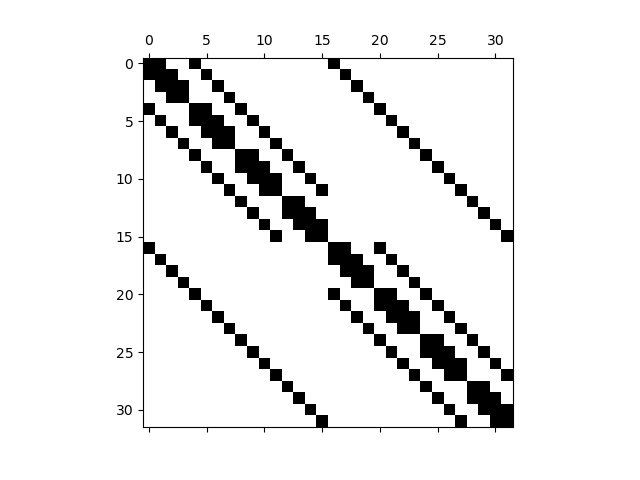
\includegraphics[scale=1.0]{img/spy4.png}
\end{figure}

The size of the resulting matrix scales very rapidly with the domain discretization. A \(100 \times 100\) domain discretization results in a \(20000 \times 20000\) sparse mass matrix to be solved with a direct solution method. For reference, the data visualization of such a matrix looks as seen in the image below, representing an incredibly sparse numerical pattern:

\begin{figure}[H]
    \centering
    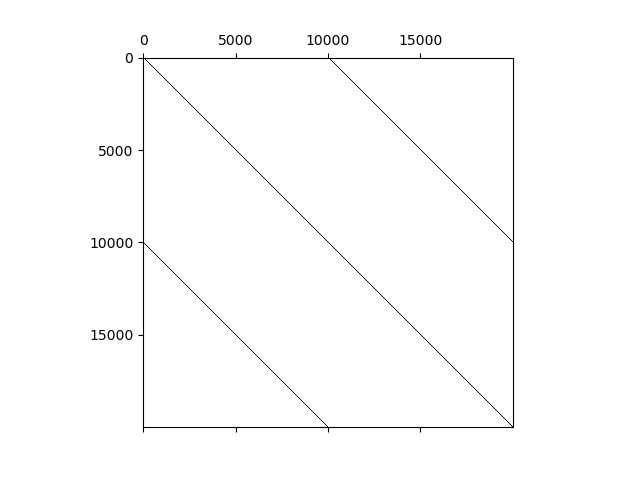
\includegraphics[scale=1.0]{img/spy100.png}
\end{figure}

An iterative solution method may be possible, but typically requires a preconditioned problem and such numerical studies are likely to be outside the scope of the current research domain.

%%%%%%%%%%%%%%%%%%%%%%%%%%%%%%%%%%%%%%%%%%%%%%%%%%%%%%%%%%%%%%%%%%%%%%%%%%%%%%%

\newpage
\section*{One-Dimensional Galerkin Finite Element}

The defining physics of this system are governed by the following equations with a temperature-independent specific heat and density:

\begin{equation*}
    \frac{1}{c} \frac{\partial}{\partial t} \Phi\left(t\right) + \sigma_a\left(T, t\right) \Phi\left(t\right) = c \sigma_a\left(T, t\right) a T^4\left(t\right)
\end{equation*}

\begin{equation*}
    \rho c_v \frac{\partial}{\partial t} T\left(t\right) + c \sigma_a \left(T, t\right) a T^4\left(t\right) = \sigma_a\left(T, t\right) \Phi\left(t\right)
\end{equation*}

Subject to initial conditions:

\begin{equation*}
    \Phi\left(0\right) = \Phi_0 \quad , \quad T\left(0\right) = T_0
\end{equation*}

Sum the equations:

\begin{equation*}
    \frac{\partial}{\partial t} \left[ \frac{1}{c} \phi\left(t\right) + \rho c_v T\left(t\right)\right] = 0
\end{equation*}

This means that the terms in the time-derivative are constant:

\begin{equation*}
    \Phi\left(t\right) + c \rho c_v T\left(t\right) = E_0
\end{equation*}

Due to the lack of a source or sink of energy in these equations, \(\phi\) and \(T\) are perfectly correlated.

\begin{equation*}
    T\left(t\right) = \frac{1}{c \rho c_v} \left[E_0 - \Phi\left(t\right)\right]
\end{equation*}

The joint conditional probability density them simplifies to:

\begin{equation*}
    P_i\left(\phi, \theta, t\right) = P_i\left(\phi, t\right) \delta\left[\theta - \frac{1}{c \rho c_v} \left(E_0 - \phi\right)\right]
\end{equation*}

The conservation of probability results in:

\begin{equation*}
    \frac{\partial}{\partial t} \left(p_1 P_1\right) + \frac{\partial}{\partial \phi} \left(\overline{f}_1 p_1 P_1\right) = \frac{p_2}{\tau_2} P_2 - \frac{p_1}{\tau_1} P_1
\end{equation*}

\begin{equation*}
    \frac{\partial}{\partial t} \left(p_2 P_2\right) + \frac{\partial}{\partial \phi} \left(\overline{f}_2 p_2 P_2\right) = \frac{p_1}{\tau_1} P_1 - \frac{p_2}{\tau_2} P_2
\end{equation*}

Subject to the initial condition:

\begin{equation*}
    P_i \left(\phi, \theta, 0\right) = \delta\left(\phi - \phi_0\right)
\end{equation*}

With the non-constant coefficients of:

\begin{equation*}
    \overline{f}_i \left(\phi\right) = c \sigma_{ai} \left[\theta\left(\phi\right)\right] \left[c a \theta^4\left(\phi\right) - \phi\right]
\end{equation*}

Where the temperature value is in terms of the radiation intensity:

\begin{equation*}
    \theta\left(\phi\right) = \frac{1}{c \rho c_v} \left(E_0 - \phi\right)
\end{equation*}

The finite element approximation involving a basis function is applied, using a notational shorthand for the non-constant coefficient terms combined with the joint conditional probability of interest, again writing \(p_i P_i\) as simply \(P_i\) for brevity:

\begin{equation*}
    F = \overline{f}_1 P_1 \quad , \quad G = \overline{f}_2 P_2
\end{equation*}

\begin{equation*}
    \int_\phi b_i\left(\phi\right)\left[ \frac{\partial P_1}{\partial t} + \frac{\partial F}{\partial \phi} = \frac{1}{\tau_2} P_2 - \frac{1}{\tau_1} P_1\right] d\phi
\end{equation*}

\begin{equation*}
    \int_\phi b_i\left(\phi\right) \left[\frac{\partial P_2}{\partial t} + \frac{\partial G}{\partial \phi} = \frac{1}{\tau_1} P_1 - \frac{1}{\tau_2} P_2 \right] d\phi
\end{equation*}

The finite element method will be derived using the Lagrange polynomials as basis functions. Integrating the non-constant coefficients by parts within a discretized cell in the \(\phi\) dimension between the upper value \(\phi_U\) and the lower value \(\phi_L\) results in the weak-form solution:

\begin{equation*}
    b_i\left(\phi\right) \hat{F}\left(\phi\right) |_{\phi_L}^{\phi_U} - \int_{\phi_L}^{\phi_U} b_i^\prime\left(\phi\right) F\left(\phi\right) d\phi
\end{equation*}

\begin{equation*}
    b_i\left(\phi\right) \hat{G}\left(\phi\right) |_{\phi_L}^{\phi_U} - \int_{\phi_L}^{\phi_U} b_i^\prime\left(\phi\right) G\left(\phi\right) d\phi
\end{equation*}

For the first parts of these terms, applying two orders of Lagrangian basis functions:

\begin{align*}
    b_1\left(\phi\right) &= \frac{\phi_U - \phi}{\phi_U - \phi_L} \\
    b_1\left(\phi_L\right) &= 1 \\
    b_1\left(\phi_U\right) &= 0 \\
    b_2\left(\phi\right) &= \frac{\phi - \phi_L}{\phi_U - \phi_L} \\
    b_2\left(\phi_L\right) &= 0 \\
    b_2\left(\phi_U\right) &= 1
\end{align*}

\begin{equation*}
    b_1\left(\phi_U\right) \hat{F}^1_{i}\left(\phi_U\right) - b_1\left(\phi_L\right) \hat{F}^1_{i}\left(\phi_L\right) = - \hat{F}^1_{i}\left(\phi_L\right)
\end{equation*}

\begin{equation*}
    b_2\left(\phi_U\right) \hat{F}^2_i\left(\phi_U\right) - b_2\left(\phi_L\right) \hat{F}^2_{i}\left(\phi_L\right) = \hat{F}^2_i\left(\phi_U\right)
\end{equation*}

\begin{equation*}
    b_1\left(\phi_U\right) \hat{G}^1_{i}\left(\phi_U\right) - b_1\left(\phi_L\right) \hat{G}^1_i\left(\phi_L\right) = - \hat{G}^1_i\left(\phi_L\right)
\end{equation*}

\begin{equation*}
    b_2\left(\phi_U\right) \hat{G}^2_{i}\left(\phi_U\right) - b_2\left(\phi_L\right) \hat{G}^2_i\left(\phi_L\right) = \hat{G}^2_{i} \left(\phi_U\right)
\end{equation*}

Note that the upwinding direction in the material 1 \(F\) terms is forwards within cell \(i\), and the upwinding direction in the material 2 \(G\) terms is backwards within cell \(i\):

\begin{align*}
    \hat{F}^1_i\left(\phi_L\right) &= \hat{F}^2_{i-1}\left(\phi_U\right) = \overline{f}_1\left(\phi_{U,i-1}\right) P^{2}_{i-1} \\
    \hat{F}^2_i\left(\phi_U\right) &= \hat{F}^2_{i}\left(\phi_U\right) = \overline{f}_1\left(\phi_{U,i}\right) P^{2}_{i} \\
    \hat{G}^1_i\left(\phi_L\right) &= \hat{G}^1_i\left(\phi_L\right) = \overline{f}_2\left(\phi_{L,i}\right) P^1_i \\
    \hat{G}^2_i\left(\phi_U\right) &= \hat{G}^1_{i+1}\left(\phi_U\right) = \overline{f}_2\left(\phi_{L,i+1}\right) P^1_{i+1}
\end{align*}

For the second part of these equations, the integral terms may simply be represented by the variables \(V\) and \(W\) for now as they are able to be algebraically and/or numerically computed prior to the solution.

\begin{equation*}
    \int_{\phi_L}^{\phi_U} b_1^\prime\left(\phi\right) F\left(\phi\right) d\phi = V_1
\end{equation*}

\begin{equation*}
    \int_{\phi_L}^{\phi_U} b_2^\prime\left(\phi\right) F\left(\phi\right) d\phi = V_2
\end{equation*}

\begin{equation*}
    \int_{\phi_L}^{\phi_U} b_1^\prime \left(\phi\right) G\left(\phi\right) d\phi = W_1
\end{equation*}

\begin{equation*}
    \int_{\phi_L}^{\phi_U} b_2^\prime\left(\phi\right) G\left(\phi\right) d\phi = W_2
\end{equation*}

Therefore resulting in:

\begin{equation*}
    \int_{\phi_L}^{\phi_U} \frac{\partial F}{\partial \phi} d\phi =
    \begin{bmatrix}
        - \overline{f}_1\left(\phi_{U,i-1}\right)P^2_{i-1} - V_1 \\
        \overline{f}_1\left(\phi_{U,i}\right)P^2_{i} - V_2
    \end{bmatrix}
\end{equation*}

\begin{equation*}
    \int_{\phi_L}^{\phi_U} \frac{\partial G}{\partial \phi} d\phi =
    \begin{bmatrix}
        -\overline{f}_2\left(\phi_{L,i}\right)P^1_i - W_1 \\
        \overline{f}_2\left(\phi_{L,i+1}\right)P^1_{i+1} - W_2
    \end{bmatrix}
\end{equation*}

As the function is the sum of the basis multiplier terms:

\begin{equation*}
    F\left(\phi\right) = \left(\overline{f}_1\left(\phi\right) P_1\right) b_1\left(\phi\right) + \left(\overline{f}_1\left(\phi\right) P_1\right) b_2\left(\phi\right)
\end{equation*}

\begin{equation*}
    G\left(\phi\right) = \left(\overline{f}_2\left(\phi\right) P_2\right) b_1\left(\phi\right) + \left(\overline{f}_2\left(\phi\right) P_2\right) b_2\left(\phi\right)
\end{equation*}

For the terms with the constant coefficients, it suffices to focus on one expression of such, using a generic variable for \(P\) without subscripts. For a second-order Lagrangian basis function application, this becomes the following equation, expressing the joint conditional probability densities in terms of second-order constants:

\begin{equation*}
    \int_{\phi_L}^{\phi_U} P d\phi = \frac{\phi_U - \phi_L}{3}
    \begin{bmatrix}
        2 & 1\\
        1 & 2
    \end{bmatrix}
    \begin{bmatrix}
        P^1 \\
        P^2
    \end{bmatrix}
\end{equation*}

The temporal derivative will have an implicit Eulerian discretization imposed on it with index \(n\):

\begin{equation*}
    \frac{\partial P}{\partial t} = \frac{1}{\Delta t} \left(P^{n+1} - P^n\right)
\end{equation*}

Applied to the joint conditional probability density equations with an Eulerian time-step discretization, the result is:

\begin{multline*}
    \int_\phi b_i\left(\phi\right) \left[\frac{\partial P_1}{\partial t} + \frac{\partial F}{\partial \phi} = \frac{1}{\tau_2} P_2 - \frac{1}{\tau_1} P_1 \right] d\phi \implies \\
    \frac{\Delta \phi}{3}
    \begin{bmatrix}
        2 & 1 \\
        1 & 2
    \end{bmatrix}
    \begin{bmatrix}
        P_{1,i}^1 \\
        P_{1,i}^2
    \end{bmatrix}^{n+1}
    + \Delta t
    \begin{bmatrix}
        - \overline{f}_1\left(\phi_{U,i-1}\right) P^2_{1,i-1} - V_1 \\
        \overline{f}_1\left(\phi_{U,i}\right) P^2_{1,i} - V_2
    \end{bmatrix}^{n+1}
    + \frac{\Delta t \Delta \phi}{3 \tau_1}
    \begin{bmatrix}
        2 & 1 \\
        1 & 2
    \end{bmatrix}
    \begin{bmatrix}
        P_{1,i}^1 \\
        P_{1,i}^2
    \end{bmatrix}^{n+1} \\
    - \frac{\Delta t \Delta \phi}{3 \tau_2}
    \begin{bmatrix}
        2 & 1 \\
        1 & 2
    \end{bmatrix}
    \begin{bmatrix}
        P_{2,i}^1 \\
        P_{2,i}^1
    \end{bmatrix}^{n+1}
    = \frac{\Delta \phi}{3}
    \begin{bmatrix}
        2 & 1 \\
        1 & 2
    \end{bmatrix}
    \begin{bmatrix}
        P_{1,i}^1 \\
        P_{1,i}^2
    \end{bmatrix}^n
    \implies \\
    \frac{\Delta \phi}{3}\left(1 + \frac{\Delta t}{\tau_1}\right)
    \begin{bmatrix}
        2 & 1 \\
        1 & 2
    \end{bmatrix}
    \begin{bmatrix}
        P^1_{1,i} \\
        P^2_{1,i}
    \end{bmatrix}^{n+1}
    + \Delta t
    \begin{bmatrix}
        - \overline{f}_1\left(\phi_{U,i-1}\right) P^2_{1,i-1} - V_1 \\
        \overline{f}_1\left(\phi_{U,i}\right) P^2_{1,i} - V_2
    \end{bmatrix}^{n+1} \\
    - \frac{\Delta t \Delta \phi}{3 \tau_2}
    \begin{bmatrix}
        2 & 1 \\
        1 & 2
    \end{bmatrix}
    \begin{bmatrix}
        P_{2,i}^1 \\
        P_{2,i}^1
    \end{bmatrix}^{n+1}
    = \frac{\Delta \phi}{3}
    \begin{bmatrix}
        2 & 1 \\
        1 & 2
    \end{bmatrix}
    \begin{bmatrix}
        P_{1,i}^1 \\
        P_{1,i}^2
    \end{bmatrix}^n
\end{multline*}

And similarly for Material 2:

\begin{multline*}
    \int_\phi b_i\left(\phi\right) \left[ \frac{\partial P_2}{\partial t} + \frac{\partial G}{\partial \phi} = \frac{1}{\tau_1} P_1 - \frac{1}{\tau_2} P_2\right] d\phi \implies \\
    \frac{\Delta \phi}{3}\left(1 + \frac{\Delta t}{\tau_2}\right)
    \begin{bmatrix}
        2 & 1 \\
        1 & 2
    \end{bmatrix}
    \begin{bmatrix}
        P^1_{2,i} \\
        P^2_{2,i}
    \end{bmatrix}^{n+1}
    + \Delta t
    \begin{bmatrix}
        - \overline{f}_2\left(\phi_{L,i}\right) P^1_{2,i} - W_1 \\
        \overline{f}_2\left(\phi_{L,i+1}\right) P^1_{2,i+1} - W_2
    \end{bmatrix}^{n+1} \\
    - \frac{\Delta t \Delta \phi}{3 \tau_1}
    \begin{bmatrix}
        2 & 1 \\
        1 & 2
    \end{bmatrix}
    \begin{bmatrix}
        P_{1,i}^1 \\
        P_{1,i}^1
    \end{bmatrix}^{n+1}
    = \frac{\Delta \phi}{3}
    \begin{bmatrix}
        2 & 1 \\
        1 & 2
    \end{bmatrix}
    \begin{bmatrix}
        P_{2,i}^1 \\
        P_{2,i}^2
    \end{bmatrix}^n
\end{multline*}

These terms result in a block lower diagonal matrix for Material 1 in the cell index \(i\), and a block upper diagonal matrix for Material 2 in the cell index \(i\). Taking into account the upwinding schemes, these block diagonal matrices are combined into a tridiagonal matrix structure over the discretization in \(\phi\). However, these terms may be best computed in a Jacobi or Gauss-Seidel convergence scheme. Some pseudocode for such a scheme is presented, using \(n\) as a time-step index and \(k\) as an iteration index:

\begin{algorithm}[H]
    \caption*{Jacobi Iteration}
    \begin{algorithmic}
        \REQUIRE Initial Conditions
        \FOR{\(t = 1:T\)}
            \STATE Guess \(P_1^{n+1,k}\), \(P_2^{n+1, k}\)
            \WHILE{Not Converged}
                \STATE Solve for \(P_1^{n+1, k+1}\) with lagged \(P_2^{n+1,k}\)
                \STATE Solve for \(P_2^{n+1, k+1}\) with lagged \(P_1^{n+1,k}\)
                \STATE Compute error, check for convergence
            \ENDWHILE
        \ENDFOR
    \end{algorithmic}
\end{algorithm}

Where the means of computing the joint conditional probability terms are detailed below. Values resulting from numerical integration are represented by the symbol \(x\):

\begin{algorithm}[H]
    \caption*{Solve for \(P_1^{n+1,k+1}\) with lagged \(P_2^{n+1,k}\)}
    \begin{algorithmic}
        \FOR{\(i = 1:I\)}
            \STATE Compute source terms:
            \begin{multline*}
                \begin{bmatrix}
                    s^1 \\
                    s^2
                \end{bmatrix}
                = \frac{\Delta \phi}{3}
                \begin{bmatrix}
                    2 & 1 \\
                    1 & 2
                \end{bmatrix}
                \begin{bmatrix}
                    P_{1,i}^{1,n,k+1} \\
                    P_{1,i}^{2,n,k+1}
                \end{bmatrix}
                + \frac{\Delta t \Delta \phi}{3 \tau_2}
                \begin{bmatrix}
                    2 & 1 \\
                    1 & 2
                \end{bmatrix}
                \begin{bmatrix}
                    P_{2,i}^{1,n+1,k} \\
                    P_{2,i}^{2,n+1,k}
                \end{bmatrix} \\
                +
                \begin{bmatrix}
                    0 & \overline{f}_1\left(\phi_{U,i-1}\right) \\
                    0 & 0
                \end{bmatrix}
                \begin{bmatrix}
                    P_{1,i-1}^{1,n+1,k+1} \\
                    P_{1,i-1}^{2,n+1,k+1}
                \end{bmatrix}
            \end{multline*}
            \STATE Solve:
            \begin{equation*}
                \left\{\frac{\Delta \phi}{3}\left(1 + \frac{\Delta t}{\tau_1}\right)
                \begin{bmatrix}
                    2 & 1 \\
                    1 & 2
                \end{bmatrix}
                + \Delta t
                \begin{bmatrix}
                    x & x \\
                    x & x
                \end{bmatrix}
                \right\}
                \begin{bmatrix}
                    P_{1,i}^{1,n+1,k+1} \\
                    P_{1,i}^{2,n+1,k+1}
                \end{bmatrix}
                =
                \begin{bmatrix}
                    s^1 \\
                    s^2
                \end{bmatrix}
            \end{equation*}
            \STATE Update \(P_1\)
        \ENDFOR
    \end{algorithmic}
\end{algorithm}

And similarly for the \(P_2\) terms, where values resulting from numerical integration are represented by the symbol \(y\):

\begin{algorithm}[H]
    \caption*{Solve for \(P_2^{n+1,k+1}\) with lagged \(P_1^{n+1,k}\)}
    \begin{algorithmic}
        \FOR{\(i=1:I\)}
            \STATE Compute source terms:
            \begin{multline*}
                \begin{bmatrix}
                    s^1 \\
                    s^2
                \end{bmatrix}
                = \frac{\Delta \phi}{3}
                \begin{bmatrix}
                    2 & 1 \\
                    1 & 2
                \end{bmatrix}
                \begin{bmatrix}
                    P_{2,i}^{1,n,k+1} \\
                    P_{2,i}^{2,n,k+1}
                \end{bmatrix}
                + \frac{\Delta t \Delta \phi}{3 \tau_1}
                \begin{bmatrix}
                    2 & 1 \\
                    1 & 2
                \end{bmatrix}
                \begin{bmatrix}
                    P_{1,i}^{1,n+1,k} \\
                    P_{1,i}^{2,n+1,k}
                \end{bmatrix} \\
                +
                \begin{bmatrix}
                    0 & 0 \\
                    -\overline{f}_2\left(\phi_{L,i+1}\right) & 0
                \end{bmatrix}
                \begin{bmatrix}
                    P_{2,i+1}^{1,n+1,k+1} \\
                    P_{2,i+1}^{2,n+1,k+1}
                \end{bmatrix}
            \end{multline*}
            \STATE Solve:
            \begin{equation*}
                \left\{ \frac{\Delta \phi}{3} \left(1 + \frac{\Delta t}{\tau_2}\right)
                \begin{bmatrix}
                    2 & 1 \\
                    1 & 2
                \end{bmatrix}
                + \Delta t
                \begin{bmatrix}
                    y & y \\
                    y & y
                \end{bmatrix}
                \right\}
                \begin{bmatrix}
                    P_{2,i}^{1,n+1,k+1} \\
                    P_{2,i}^{2,n+1,k+1}
                \end{bmatrix}
                =
                \begin{bmatrix}
                    s^1 \\
                    s^2
                \end{bmatrix}
            \end{equation*}
        \ENDFOR
    \end{algorithmic}
\end{algorithm}

On the terms resulting from numerical integration, these will look as follows:

\begin{multline*}
    V_1 = \int_{\phi_L}^{\phi_U} b_1^\prime\left(\phi\right) F\left(\phi\right) d\phi = \int_{\phi_L}^{\phi_U} b_1^\prime \left[ \sum_{r=1}^{2} b_r \left(\phi\right) b_1^\prime\left(\phi\right) \overline{f}_1\left(\phi\right) P_1^r \right] d\phi = \\
    P_1^1 \int_{\phi_L}^{\phi_U} b_1\left(\phi\right) b_1^\prime\left(\phi\right) \overline{f}_1\left(\phi\right) d\phi + P_1^2 \int_{\phi_L}^{\phi_U} b_2\left(\phi\right) b_1^\prime \left(\phi\right) \overline{f}_1\left(\phi\right) d\phi
\end{multline*}

\begin{multline*}
    V_2 = \int_{\phi_L}^{\phi_U} b_2^\prime\left(\phi\right) F\left(\phi\right) = \int_{\phi_L}^{\phi_U} b_2^\prime\left[\sum_{r=1}^2 b_r \left(\phi\right) b_2^\prime\left(\phi\right) \overline{f}_1\left(\phi\right) P_1^r\right] d\phi = \\
    P_1^1 \int_{\phi_L}^{\phi_U} b_1\left(\phi\right) b_2^\prime\left(\phi\right) \overline{f}_1\left(\phi\right) d\phi + P_1^2 \int_{\phi_L}^{\phi_U} b_2\left(\phi\right) b_2^\prime \left(\phi\right) \overline{f}_1\left(\phi\right) d\phi
\end{multline*}

\begin{multline*}
    W_1 = \int_{\phi_L}^{\phi_U} b_1^\prime\left(\phi\right) G\left(\phi\right) d\phi = \int_{\phi_L}^{\phi_U} b_1^\prime \left[ \sum_{r=1}^{2} b_r \left(\phi\right) b_1^\prime\left(\phi\right) \overline{f}_2\left(\phi\right) P_2^r \right] d\phi = \\
    P_2^1 \int_{\phi_L}^{\phi_U} b_1\left(\phi\right) b_1^\prime\left(\phi\right) \overline{f}_2\left(\phi\right) d\phi + P_2^2 \int_{\phi_L}^{\phi_U} b_2\left(\phi\right) b_1^\prime \left(\phi\right) \overline{f}_2\left(\phi\right) d\phi
\end{multline*}

\begin{multline*}
    W_2 = \int_{\phi_L}^{\phi_U} b_2^\prime\left(\phi\right) G\left(\phi\right) d\phi = \int_{\phi_L}^{\phi_U} b_2^\prime \left[ \sum_{r=1}^{2} b_r \left(\phi\right) b_2^\prime\left(\phi\right) \overline{f}_2\left(\phi\right) P_2^r \right] d\phi = \\
    P_2^1 \int_{\phi_L}^{\phi_U} b_1\left(\phi\right) b_2^\prime\left(\phi\right) \overline{f}_2\left(\phi\right) d\phi + P_2^2 \int_{\phi_L}^{\phi_U} b_2\left(\phi\right) b_2^\prime \left(\phi\right) \overline{f}_2\left(\phi\right) d\phi
\end{multline*}

Meaning that the placeholder terms in the pseudocode algorithm look as follows:

\begin{multline*}
    \begin{bmatrix}
        x & x \\
        x & x
    \end{bmatrix}
    \begin{bmatrix}
        P_1^1 \\
        P_1^2
    \end{bmatrix}
    = \\
    \begin{bmatrix}
        - \int_{\phi_L}^{\phi_U} b_1\left(\phi\right) b_1^\prime\left(\phi\right) \overline{f}_1\left(\phi\right) d\phi & - \int_{\phi_L}^{\phi_U} b_2\left(\phi\right) b_1^\prime\left(\phi\right) \overline{f}_1\left(\phi\right) d\phi \\
        - \int_{\phi_L}^{\phi_U} b_1\left(\phi\right) b_2^\prime\left(\phi\right) \overline{f}_1\left(\phi\right) d\phi & \overline{f}_1\left(\phi_{U,i}\right) - \int_{\phi_L}^{\phi_U} b_2\left(\phi\right) b_2^\prime\left(\phi\right) \overline{f}_1\left(\phi\right) d\phi
    \end{bmatrix}
    \begin{bmatrix}
        P_1^1 \\
        P_1^2
    \end{bmatrix}
\end{multline*}

\begin{multline*}
    \begin{bmatrix}
        y & y \\
        y & y
    \end{bmatrix}
    \begin{bmatrix}
        P_2^1 \\
        P_2^2
    \end{bmatrix}
    = \\
    \begin{bmatrix}
        - \overline{f}_2\left(\phi_{L,i}\right) - \int_{\phi_L}^{\phi_U} b_1\left(\phi\right) b_1^\prime\left(\phi\right) \overline{f}_2\left(\phi\right) d\phi & - \int_{\phi_L}^{\phi_U} b_2\left(\phi\right) b_1^\prime\left(\phi\right) \overline{f}_2\left(\phi\right) d\phi \\
        - \int_{\phi_L}^{\phi_U} b_1\left(\phi\right) b_2^\prime\left(\phi\right) \overline{f}_2\left(\phi\right) d\phi & -\int_{\phi_L}^{\phi_U} b_2\left(\phi\right) b_2^\prime \left(\phi\right) \overline{f}_2\left(\phi\right) d\phi
    \end{bmatrix}
    \begin{bmatrix}
        P_2^1 \\
        P_2^2
    \end{bmatrix}
\end{multline*}

%%%%%%%%%%%%%%%%%%%%%%%%%%%%%%%%%%%%%%%%%%%%%%%%%%%%%%%%%%%%%%%%%%%%%%%%%%%%%%

\newpage
\section*{Two-Dimensional Galerkin Finite Element}
To facilitate the Galerkin finite element solution, we can rewrite the original equations leaving off the dependence on \(\phi\), \(\theta\), and \(t\) for brevity:

\begin{equation*}
    \frac{\partial P_1}{\partial t} + \frac{\partial f_1 P_1}{\partial \phi} + \frac{\partial g_1 P_1}{\partial \theta} + \frac{1}{\tau_1} P_1 = \frac{1}{\tau_2} P_2
\end{equation*}

\begin{equation*}
    \frac{\partial P_2}{\partial t} + \frac{\partial f_2 P_2}{\partial \phi} + \frac{\partial g_2 P_2}{\partial \theta} + \frac{1}{\tau_2} P_2 = \frac{1}{\tau_1} P_1
\end{equation*}

We begin by establishing the equations for a finite element discretization of the probability including basis functions \(v\left(\phi\right)\) and \(w\left(\theta\right)\):

\begin{equation*}
    P_1 = \sum_i v_i\left(\phi\right) \sum_j w_j\left(\theta\right) P_1^{i,j}
\end{equation*}

\begin{equation*}
    P_2  = \sum_i v_i\left(\phi\right) \sum_j w_j\left(\theta\right) P_2^{i,j}
\end{equation*}

The linear model of probability, using linear basis functions wherein the zeroeth-order term is equivalent to unity, would then look as:

\begin{equation*}
    P_1 = P_1^{0,0} + v_1\left(\phi\right) P_1^{1,0} + w_1\left(\theta\right) P_1^{0,1} + v_1\left(\phi\right) w_1\left(\theta\right) P_1^{1,1}
\end{equation*}

\begin{equation*}
    P_2 = P_2^{0,0} + v_1\left(\phi\right) P_2^{1,0} + w_1\left(\theta\right) P_2^{0,1} + v_1\left(\phi\right) w_1\left(\theta\right) P_2^{1,1}
\end{equation*}

For comparison, the second-order equations are also presented, though further analysis will make use of the linear model for ease of computation:

\begin{align*}
    P_1 = & v_2\left(\phi\right) \left[w_0\left(\theta\right) P_1^{2,0} + w_1\left(\theta\right) P_1^{2,1} + w_2\left(\theta\right) P_1^{2,2}\right] + \\
    & v_1\left(\phi\right) \left[w_0\left(\theta\right) P_1^{2,0} + w_1\left(\theta\right) P_1^{2,1} + w_2\left(\theta\right) P_1^{2,2}\right] + \\
    & v_0\left(\phi\right) \left[w_0\left(\theta\right) P_1^{2,0} + w_1\left(\theta\right) P_1^{2,1} + w_2\left(\theta\right) P_1^{2,2}\right]
\end{align*}

\begin{align*}
    P_2 = & v_2\left(\phi\right) \left[w_0\left(\theta\right) P_2^{2,0} + w_1\left(\theta\right) P_2^{2,1} + w_2\left(\theta\right) P_2^{2,2}\right] + \\
    & v_1\left(\phi\right) \left[w_0\left(\theta\right) P_2^{2,0} + w_1\left(\theta\right) P_2^{2,1} + w_2\left(\theta\right) P_2^{2,2}\right] + \\
    & v_0\left(\phi\right) \left[w_0\left(\theta\right) P_2^{2,0} + w_1\left(\theta\right) P_2^{2,1} + w_2\left(\theta\right) P_2^{2,2}\right]
\end{align*}

Substituting the equation for the probability into the master equations underneath the finite element integration scheme, using \(P\) as a material-agnostic representation of \(P_1\) and \(P_2\), and \(\tau\) as a material-agnostic representation of \(\tau_1\) and \(\tau_2\):

\begin{multline*}
    \int_\phi \int_\theta v\left(\phi\right) w\left(\theta\right) \frac{1}{\tau} P d\phi d\theta = \\
    \int_\phi \int_\theta v\left(\phi\right) w\left(\theta\right) \frac{1}{\tau} \left[P^{0,0} + v_1\left(\phi\right) P^{1,0} + w_1\left(\theta\right) P^{0,1} + v_1\left(\phi\right) w_1\left(\theta\right) P^{1,1}\right] d\theta d\phi
\end{multline*}

For the first step, using the zeroeth-order forms of \(v\) and \(w\), where the subscripts on the domain represent the lower bounds and upper-bounds as \(L\) and \(U\) respectively:

\begin{equation*}
    \int_{\phi_L}^{\phi_U} \int_{\theta_L}^{\theta_U} v_0\left(\phi\right) w_0\left(\theta\right) \frac{1}{\tau} P d\theta d\phi
\end{equation*}

As \(v_0\) and \(w_0\) are both constants equal to unity, the Legendre coefficients in this integral become straightforward:

\begin{multline*}
    \int_{\phi_L}^{\phi_U} \int_{\theta_L}^{\theta_U} \frac{1}{\tau} P d\theta d\phi = \\
    \frac{1}{\tau} \int_{\phi_L}^{\phi_U} \int_{\theta_L}^{\theta_U} \left[P^{0,0} + v_1\left(\phi\right) P^{1,0} + w_1\left(\phi\right) P^{0,1} + v_1\left(\phi\right) w_1\left(\phi\right) P^{1,1}\right] d\theta d\phi
\end{multline*}

Bearing in mind that the Legendre Polynomials maintain orthogonality on the domain of \(\left[-1, 1\right]\) within the confines of each cell, we can allow for the domain substitution to occur transforming \(\phi\) and \(\theta\) for these basis functions to exist and maintain orthogonality within this domain:

\begin{align*}
    \phi & = \frac{2}{\phi_U - \phi_L} \left(\phi - \frac{\phi_U + \phi_L}{2}\right) \\
    \theta & = \frac{2}{\theta_U - \theta_L} \left(\theta - \frac{\theta_U + \theta_L}{2}\right)
\end{align*}

This is useful, as the first-order Legendre polynomials \(v_1\) and \(w_1\) are equal to \(\phi\) and \(\theta\), respectively:

\begin{align*}
    \int_{\phi_L}^{\phi_U} \int_{\theta_L}^{\theta_U} P d\theta d\phi & = \\
    & \int_{\phi_L}^{\phi_U} \int_{\theta_L}^{\theta_U} P^{0,0} d\theta d\phi \\
    & + \int_{\phi_L}^{\phi_U} \int_{\theta_L}^{\theta_U} \left[\frac{2}{\phi_U - \phi_L} \left(\phi - \frac{\phi_U + \phi_L}{2}\right) P^{1,0}\right] d\theta d\phi \\
    & + \int_{\phi_L}^{\phi_U} \int_{\theta_L}^{\theta_U} \left[\frac{2}{\theta_U - \theta_L} \left(\theta - \frac{\theta_U + \theta_L}{2}\right) P^{0,1}\right] d\theta d\phi \\
    & + \int_{\phi_L}^{\phi_U} \int_{\theta_L}^{\theta_U} \left[\frac{2}{\phi_U - \phi_L} \left(\phi - \frac{\phi_U + \phi_L}{2}\right) \frac{2}{\theta_U - \theta_L} \left(\theta - \frac{\theta_U + \theta_L}{2}\right) P^{1,1}\right] d\theta d\phi
\end{align*}

Term-by-term solutions:

\begin{equation*}
    \int_{\phi_L}^{\phi_U} \int_{\theta_L}^{\theta_U} P^{0,0} d\theta d\phi = \left(\phi_U - \phi_L\right) \left(\theta_U - \theta_L\right) P^{0,0}
\end{equation*}

\begin{equation*}
    \int_{\phi_L}^{\phi_U} \int_{\theta_L}^{\theta_U} \left[\frac{2}{\phi_U - \phi_L} \left(\phi - \frac{\phi_U + \phi_L}{2}\right) P^{1,0} \right] d\theta d\phi = 0
\end{equation*}

\begin{equation*}
    \int_{\phi_L}^{\phi_U} \int_{\theta_L}^{\theta_U} \left[\frac{2}{\theta_U - \theta_L} \left(\theta - \frac{\theta_U + \theta_L}{2}\right) P^{0,1} \right] d\theta d\phi = 0
\end{equation*}

\begin{equation*}
    \int_{\phi_L}^{\phi_U} \int_{\theta_L}^{\theta_U}  \left[\frac{2}{\phi_U - \phi_L} \left(\phi - \frac{\phi_U + \phi_L}{2}\right) \frac{2}{\theta_U - \theta_L} \left(\theta - \frac{\theta_U + \theta_L}{2}\right) P^{1,1}\right] d\theta d\phi = 0
\end{equation*}

The zero-terms come about due to the orthogonality property of Legendre polynomials. The end result of this term is:

\begin{equation*}
    \int_\phi \int_\theta v_0\left(\phi\right) w_0\left(\theta\right) P d\theta d\phi = \boxed{\left(\phi_U - \phi_L\right) \left(\theta_U - \theta_L\right) P^{0,0}}
\end{equation*}

The next evaluation:

\begin{align*}
    \int_\phi \int_\theta v_1\left(\phi\right) w_0\left(\theta\right) P d\theta d\phi &= \int_\phi \int_\theta \phi \left[P^{0,0} + \phi P^{1,0} + \theta P^{0,1} + \phi \theta P^{1,1} \right] d\theta d\phi \\
    & = \int_\phi \int_\theta \left[\phi P^{0,0} + \phi^2 P^{1,0} + \phi \theta P^{0,1} + \phi^2 \theta P^{1,1}\right] d\theta d\phi
\end{align*}

Applying the same domain substitutions, term-by-term solutions are as follows:

\begin{equation*}
    \int_{\phi_L}^{\phi_U} \int_{\theta_L}^{\theta_U} \left[\frac{2}{\phi_U - \phi_L} \left(\phi - \frac{\phi_U + \phi_L}{2}\right) P^{0,0}\right] d\theta d\phi = 0
\end{equation*}

\begin{equation*}
    \int_{\phi_L}^{\phi_U} \int_{\theta_L}^{\theta_U} \left[\left[\frac{2}{\phi_U - \phi_L} \left(\phi - \frac{\phi_U + \phi_L}{2}\right)\right]^2 P^{1,0}\right] d\theta d\phi = \frac{1}{3}\left(\phi_U - \phi_L\right) \left(\phi_U - \phi_L\right) P^{1,0}
\end{equation*}

\begin{equation*}
    \int_{\phi_L}^{\phi_U} \int_{\theta_L}^{\theta_U} \left[\frac{2}{\phi_U - \phi_L} \left(\phi - \frac{\phi_U + \phi_L}{2}\right) \frac{2}{\theta_U - \theta_L} \left(\theta - \frac{\theta_U + \theta_L}{2}\right) P^{0,1}\right] d\theta d\phi = 0
\end{equation*}

\begin{equation*}
    \int_{\phi_L}^{\phi_U} \int_{\theta_L}^{\theta_U} \left[\left[\frac{2}{\phi_U - \phi_L} \left(\phi - \frac{\phi_U + \phi_L}{2}\right)\right]^2 \frac{2}{\theta_U - \theta_L} \left(\theta - \frac{\theta_U + \theta_L}{2}\right) P^{1,1}\right] d\theta d\phi = 0
\end{equation*}

Resulting in:

\begin{equation*}
    \int_\phi \int_\theta v_1\left(\phi\right) w_1\left(\theta\right) P d\theta d\phi = \boxed{\frac{1}{3} \left(\phi_U - \phi_L\right)\left(\theta_U - \theta_L\right) P^{1,0}}
\end{equation*}

The next evaluation:

\begin{align*}
    \int_\phi \int_\theta v_0\left(\phi\right) w_1\left(\theta\right) P d\theta d\phi & = \int_\phi \int_\theta \theta \left[P^{0,0} + \phi P^{1,0} + \theta P^{0,1} + \phi \theta P^{1,1}\right] d\theta d\phi \\
    & = \int_\phi \int_\theta \left[\theta P^{0,0} + \phi \theta P^{1,0} + \theta^2 P^{0,1} + \phi \theta^2 P^{1,1}\right] d\theta d\phi
\end{align*}

Term-by-term solutions are as follows:

\begin{equation*}
    \int_{\phi_L}^{\phi_U} \int_{\theta_L}^{\theta_U} \left[\frac{2}{\theta_U - \theta_L} \left(\theta - \frac{\theta_U + \theta_L}{2}\right) P^{0,0}\right] d\theta d\phi = 0
\end{equation*}

\begin{equation*}
    \int_{\phi_L}^{\phi_U} \int_{\theta_L}^{\theta_U} \left[\frac{2}{\phi_U - \phi_L} \left(\phi - \frac{\phi_U + \phi_L}{2}\right) \frac{2}{\theta_U - \theta_L} \left(\theta - \frac{\theta_U + \theta_L}{2}\right) P^{1,0}\right] d\theta d\phi = 0
\end{equation*}

\begin{equation*}
    \int_{\phi_L}^{\phi_U} \int_{\theta_L}^{\theta_U} \left[\left[\frac{2}{\theta_U - \theta_L} \left(\theta - \frac{\theta_U + \theta_L}{2}\right)\right]^2 P^{0,1}\right] d\theta d\phi = \frac{1}{3}\left(\phi_U - \phi_L\right) \left(\theta_U - \theta_L\right) P^{0,1}
\end{equation*}

\begin{equation*}
    \int_{\phi_L}^{\phi_U} \int_{\theta_L}^{\theta_U} \left[\frac{2}{\phi_U - \phi_L} \left(\phi - \frac{\phi_U + \phi_L}{2}\right) \left[\frac{2}{\theta_U - \theta_L} \left(\theta - \frac{\theta_U + \theta_L}{2}\right)\right]^2 P^{1,0}\right] d\theta d\phi = 0
\end{equation*}

Resulting in:

\begin{equation*}
    \int_\phi \int_\theta v_0\left(\phi\right) w_1\left(\theta\right) P d\theta d\phi = \boxed{\frac{1}{3}\left(\phi_U - \phi_L\right) \left(\theta_U - \theta_L\right) P^{0,1}}
\end{equation*}

This leaves the remaining evaluation:

\begin{align*}
    \int_\phi \int_\theta v_1\left(\phi\right) w_1\left(\theta\right) P d\theta d\phi & = \int_\phi \int_\theta \phi \theta \left[ P^{0,0} + \phi P^{1,0} + \theta P^{0,1} + \phi \theta P^{1,1}\right] d\theta d\phi \\
    & = \int_\phi \int_\theta \left[ \phi \theta P^{0,0} + \phi^2 \theta P^{1,0} + \phi \theta^2 P^{0,1} + \phi^2 \theta^2 P^{1,1}\right] d\theta d\phi
\end{align*}

Term-by-term solutions are as follows:

\begin{equation*}
    \int_{\phi_L}^{\phi_U} \int_{\theta_L}^{\theta_U} \left[ \frac{2}{\phi_U - \phi_L} \left(\phi - \frac{\phi_U + \phi_L}{2}\right) \frac{2}{\theta_U - \theta_L} \left(\theta - \frac{\theta_U + \theta_L}{2}\right) P^{0,0}\right] d\theta d\phi = 0
\end{equation*}

\begin{equation*}
    \int_{\phi_L}^{\phi_U} \int_{\theta_L}^{\theta_U} \left[ \left[\frac{2}{\phi_U - \phi_L} \left(\phi - \frac{\phi_U + \phi_L}{2}\right)\right]^2 \frac{2}{\theta_U - \theta_L} \left(\theta - \frac{\theta_U + \theta_L}{2}\right) P^{1,0}\right] d\theta d\phi = 0
\end{equation*}

\begin{equation*}
    \int_{\phi_L}^{\phi_U} \int_{\theta_L}^{\theta_U} \left[ \frac{2}{\phi_U - \phi_L} \left(\phi - \frac{\phi_U + \phi_L}{2}\right) \left[\frac{2}{\theta_U - \theta_L} \left(\theta - \frac{\theta_U + \theta_L}{2}\right) \right]^2 P^{0,1}\right] d\theta d\phi = 0
\end{equation*}

\begin{multline*}
    \int_{\phi_L}^{\phi_U} \int_{\theta_L}^{\theta_U} \left[ \left[\frac{2}{\phi_U - \phi_L} \left(\phi - \frac{\phi_U + \phi_L}{2}\right)\right]^2 \left[\frac{2}{\theta_U - \theta_L} \left(\theta - \frac{\theta_U + \theta_L}{2}\right)\right]^2 P^{1,1}\right] d\theta d\phi = \\ \frac{1}{9} \left(\phi_U - \phi_L\right) \left(\theta_U - \theta_L\right) P^{1,1}
\end{multline*}

The end result of these terms is:

\begin{equation*}
    \int_\phi \int_\theta v_1\left(\phi\right) w_1\left(\theta\right) P d\theta d\phi = \boxed{\frac{1}{9} \left(\phi_U - \phi_L\right) \left(\theta_U - \theta_L\right) P^{1,1}}
\end{equation*}

For brevity, allow the term \(h = \left(\phi_U - \phi_L\right) \left(\theta_U - \theta_L\right)\) and the matrix \(\mathbf{M}\) to be defined as:

\begin{equation*}
    \mathbf{M} =
    \begin{bmatrix}
        h & 0 & 0 & 0 \\
        0 & \frac{1}{3} h & 0 & 0 \\
        0 & 0 & \frac{1}{3} h & 0 \\
        0 & 0 & 0 & \frac{1}{9} h
    \end{bmatrix}
\end{equation*}

Combining all linear terms from these expansions results in the matrix-form equation:

\begin{equation*}
    \frac{1}{\tau} P = \frac{1}{\tau} \mathbf{M}
    \begin{bmatrix}
        P^{0,0} \\
        P^{1,0} \\
        P^{0,1} \\
        P^{1,1}
    \end{bmatrix}
\end{equation*}

Analyzing the \(\phi\)-derivative term for a finite-element discretization results in:

\begin{multline*}
    \int_\phi \int_\theta v\left(\phi\right) w\left(\theta\right) \frac{\partial f\left(\phi, \theta\right) P}{\partial \phi} d\theta d\phi \\
    = \int_\phi \int_\theta v\left(\phi\right) w\left(\theta\right) \frac{\partial}{\partial \phi} f\left(\phi, \theta\right) \left[P^{0,0} + v_1\left(\phi\right) P^{1,0} + w_1\left(\theta\right) P^{0,1} + v_1\left(\phi\right) w_1\left(\theta\right) P^{1,1}\right] d\theta d\phi
\end{multline*}

Isolating one term and integrating by parts:

\begin{multline*}
    \int_\phi \int_\theta v\left(\phi\right) w\left(\theta\right) \frac{\partial \left[f\left(\phi, \theta\right) P^{0,0}\right]}{\partial \phi} d\theta d\phi \\
    = \int_\theta w\left(\theta\right) \left[ \left[ v\left(\phi\right) f\left(\phi, \theta\right) P^{0,0}\right]_{\phi_L}^{\phi_U} - \int_{\phi_L}^{\phi_U} v^\prime\left(\phi\right) f\left(\phi, \theta\right) P^{0,0}\right] d\theta
\end{multline*}

The first component, assuming \(v_0\left(\phi\right) = 1\):

\begin{multline*}
    \left[v_0\left(\phi\right) f\left(\phi, \theta\right) P^{0,0}\right]_{\phi_L}^{\phi_U} = \left[ f\left(\phi, \theta\right)P^{0,0} \right]_{\phi_L}^{\phi_U} = \left[c \sigma_a\left(\theta\right) \left(c a \theta^4 - \phi\right) P^{0,0}\right]_{\phi_L}^{\phi_U} \\
    = c \sigma_a \left(\theta\right) \left(\phi_L - \phi_U\right) P^{0,0}
\end{multline*}

Assuming \(v_1\left(\phi\right) = \phi\), and applying the dimensional transformation to the Legendre variable (but not to the non-constant coefficient terms):

\begin{multline*}
    \left[v_1\left(\phi\right) f\left(\phi,\theta\right) P^{0,0}\right]_{\phi_L}^{\phi_U} = \left[\phi f\left(\phi, \theta\right)P^{0,0}\right]_{\phi_L}^{\phi_U} = \left[\phi c \sigma_a\left(\theta\right) \left(c a \theta^4 - \phi\right) P^{0,0}\right]_{\phi_L}^{\phi_U} \\
    = \left[\frac{2}{\phi_U - \phi_L} \left(\phi - \frac{\phi_U + \phi_L}{2}\right) c \sigma_a\left(\theta\right) \left(c a \theta^4 - \phi\right) P^{0,0}\right]_{\phi_L}^{\phi_U} \\
    = \frac{2}{\phi_U - \phi_L} c \sigma_a\left(\theta\right) P^{0,0} \left[\phi c a \theta^4 - \phi^2 - c a \theta^4 \frac{\phi_U + \phi_L}{2} + \phi \frac{\phi_U + \phi_L}{2}\right]_{\phi_L}^{\phi_U} \\
    = \frac{2}{\phi_U - \phi_L} c \sigma_a\left(\theta\right) P^{0,0} \left(\phi_U c a \theta^4 - \phi_U^2 + \frac{\phi_U^2 + \phi_U \phi_L}{2} - \phi_L c a \theta^4 + \phi_L^2 - \frac{\phi_U \phi_L + \phi_L^2}{2} \right) \\
    = \frac{2}{\phi_U - \phi_L} c \sigma_a\left(\theta\right) P^{0,0} \left(c a \theta^4 \left(\phi_U - \phi_L\right) + \frac{\phi_L^2 - \phi_U^2}{2}\right) \\
    = c \sigma_a\left(\theta\right) P^{0,0} \left(2 c a \theta^4  - \phi_U - \phi_L\right)
\end{multline*}

The second component, assuming \(v_0\left(\phi\right) = 1\):

\begin{equation*}
    \int_{\phi_L}^{\phi_U} v_0^\prime\left(\phi\right) f\left(\phi, \theta\right) P^{0,0} = 0
\end{equation*}

The second component, assuming \(v_1\left(\phi\right) = \phi\), with the dimensional transformation:

\begin{multline*}
    \int_{\phi_L}^{\phi_U} v_1^\prime\left(\phi\right) f\left(\phi, \theta\right) P^{0,0} = \int_{\phi_L}^{\phi_U} \left[\frac{2}{\phi_U - \phi_L} \left(\phi - \frac{\phi_U + \phi_L}{2}\right)\right]^\prime f\left(\phi,\theta\right) P^{0,0} \\
    = \int_{\phi_L}^{\phi_U} \left(\frac{2}{\phi_U - \phi_L}\right) d \phi f \left(\phi, \theta\right) P^{0,0} = P^{0,0} \frac{2}{\phi_U - \phi_L} c \sigma_a\left(\theta\right) \int_{\phi_L}^{\phi_U} \left(c a \theta^4 - \phi\right) d \phi \\
    = P^{0,0} \frac{2}{\phi_U - \phi_L} c \sigma_a\left(\theta\right) \left[c a \theta^4 \phi - \frac{\phi^2}{2}\right]_{\phi_L}^{\phi_U} = P^{0,0} \frac{2}{\phi_U - \phi_L} c \sigma_a\left(\theta\right) \left(c a \theta^4 \left(\phi_U - \phi_L\right) + \frac{\phi_L^2 - \phi_U^2}{2}\right) \\
    = c \sigma_a\left(\theta\right) P^{0,0} \left(2 c a \theta^4 - \phi_U - \phi_L\right)
\end{multline*}

Therefore this term of the original equation results in, for \(v_0\left(\phi\right)\):

\begin{equation*}
    \int_\phi \int_\theta v_0\left(\phi\right) w\left(\theta\right) \frac{\partial \left[f \left(\phi, \theta\right) P^{0,0}\right]}{\partial \phi} d \theta d \phi = \int_\theta w\left(\theta\right) c \sigma_a\left(\theta\right) \left(\phi_L - \phi_U\right) P^{0,0} d\theta
\end{equation*}

And for \(v_1\left(\phi\right)\):

\begin{multline*}
    \int_\phi \int_\theta v_1\left(\phi\right) w\left(\theta\right) \frac{\partial \left[f \left(\phi, \theta\right) P^{0,0}\right]}{\partial \phi} d \theta d \phi = \int_\theta w\left(\theta\right) c \sigma_a\left(\theta\right) P^{0,0} \left(2 c a \theta^4 - \phi_U - \phi_L\right) d\theta \\
    - \int_\theta w\left(\theta\right) c \sigma_a\left(\theta\right) P^{0,0} \left(2 c a \theta^4 - \phi_U - \phi_L\right) d\theta = 0
\end{multline*}

The term with \(v_0\left(\phi\right)\) assuming the corresponding \(\theta\)-dimension polynomial is \(w_0\left(\theta\right) = 1\):

\begin{equation*}
    \int_\phi \int_\theta v_0\left(\phi\right) w_0\left(\theta\right) \frac{\partial \left[f\left(\phi, \theta\right)P^{0,0}\right]}{\partial \phi} d\theta d\phi = \int_{\theta_L}^{\theta_R} c \sigma_a\left(\theta\right) \left(\phi_L - \phi_U\right) P^{0,0} d \theta
\end{equation*}

Using a relationship for the opacity of the material as:

\begin{equation*}
    \sigma_a\left(\theta\right) = A \frac{1}{\theta^3}
\end{equation*}

The equation becomes:

\begin{multline*}
    \int_\phi \int_\theta v_0\left(\phi\right) w_0\left(\theta\right) \frac{\partial \left[f\left(\phi, \theta\right)P^{0,0}\right]}{\partial \phi} d\theta d\phi = cA\left(\phi_L - \phi_U\right) P^{0,0} \int_{\theta_L}^{\theta_U} \frac{1}{\theta^3} d\theta \\
    = \frac{1}{2} c A \left(\phi_L - \phi_U\right) P^{0,0} \left[-\frac{1}{\theta^2}\right]_{\theta_L}^{\theta_U} = \frac{1}{2} c A \left(\phi_L - \phi_U\right) P^{0,0} \left(\frac{1}{\theta_L^2} - \frac{1}{\theta_U^2}\right)
\end{multline*}

And assuming that the \(\theta\)-dimension polynomial is \(w_0\left(\theta\right) = \theta\):

\begin{multline*}
    \int_\phi \int_\theta v_0\left(\phi\right) w_1\left(\theta\right) \frac{\partial \left[f\left(\phi, \theta\right)P^{0,0}\right]}{\partial \phi} d\theta d\phi \\
    = \int_{\theta_L}^{\theta_R} \frac{2}{\theta_U - \theta_L}\left(\theta - \frac{\theta_U + \theta_L}{2}\right) c \sigma_a\left(\theta\right) \left(\phi_L - \phi_U\right) P^{0,0} d\theta \\
    = \frac{2}{\theta_U - \theta_L} c A \left(\phi_L - \phi_U\right) P^{0,0} \int_{\theta_L}^{\theta_U} \frac{1}{\theta^3} \left(\theta - \frac{\theta_U + \theta_L}{2}\right) d\theta \\
    = \frac{2}{\theta_U - \theta_L} c A \left(\phi_L - \phi_U\right) P^{0,0} \frac{\left(\theta_L - \theta_U\right)^3}{4 \theta_L^2 \theta_U^2}
    = c A P^{0,0} \frac{\left(\theta_L - \theta_U\right)^3\left(\phi_L - \phi_U\right)}{2 \theta_L^2 \theta_U^2 \left(\theta_U - \theta_L\right)}
\end{multline*}

While the first-order \(\phi\)-dimension Legendre polynomial coefficients drop out for the \(P^{0,0}\) terms, due to both terms being equivalent:

\begin{equation*}
    \int_\phi \int_\theta v_1\left(\phi\right) w_0\left(\theta\right) \frac{\partial \left[f\left(\phi, \theta\right) P^{0,0}\right]}{\partial \phi} d\theta d\phi = 0
\end{equation*}

\begin{equation*}
    \int_\phi \int_\theta v_{1}\left(\phi\right) w_1\left(\theta\right) \frac{\partial \left[f\left(\phi, \theta\right) P^{0,0}\right]}{\partial \phi} d\theta d\phi = 0
\end{equation*}

Therefore, for the first term in the original equation, the resulting expression is:

\begin{multline*}
    \int_\phi \int_\theta v\left(\phi\right) w\left(\theta\right) \frac{\partial\left[f\left(\phi, \theta\right) P^{0,0}\right]}{\partial \phi} d\theta d\phi \\
    = \frac{1}{2} c A P^{0,0} \left(\phi_L - \phi_U\right) \left(\frac{1}{\theta_L^2} - \frac{1}{\theta_U^2}\right) + c A P^{0,0} \frac{\left(\theta_L - \theta_U\right)^3\left(\phi_L - \phi_U\right)}{2 \theta_L^2 \theta_U^2 \left(\theta_U - \theta_L\right)} \\
    = \boxed{c A P^{0,0} \frac{\left(\phi_L - \phi_U\right) \left(\theta_U - \theta_L\right)}{\theta_L \theta_U^2}}
\end{multline*}

The second term of the original \(\phi\)-derivative substitution is integrated by parts:

\begin{multline*}
    \int_\phi \int_\theta v\left(\phi\right) w\left(\theta\right) \frac{\partial \left[v_1\left(\phi\right) f\left(\phi, \theta\right) P^{1,0}\right]}{\partial \phi} d\theta d\phi \\
    = \int_\theta w\left(\theta\right) \left[ \left[v\left(\phi\right) v_1\left(\phi\right) f\left(\phi, \theta\right) P^{1,0}\right]_{\phi_L}^{\phi_U} - \int_{\phi_L}^{\phi_U} v^\prime\left(\phi\right) v_1\left(\phi\right) f\left(\phi, \theta\right) P^{1,0} \right] d\theta
\end{multline*}

The first component, assuming \(v_0\left(\phi\right) = 1\):

\begin{multline*}
    \left[v_0\left(\phi\right) v_1\left(\phi\right) f\left(\phi, \theta\right) P^{1,0}\right]_{\phi_L}^{\phi_U} = \left[\frac{2}{\phi_U - \phi_L}\left(\phi - \frac{\phi_U + \phi_L}{2}\right) f\left(\phi, \theta\right) P^{1,0}\right]_{\phi_L}^{\phi_U} \\
    = \left[\frac{2}{\phi_U - \phi_L}\left(\phi - \frac{\phi_U + \phi_L}{2}\right) c \sigma_a\left(\theta\right) \left(c a \theta^4 - \phi\right) P^{1,0}\right]_{\phi_L}^{\phi_U} \\
    = \frac{2}{\phi_U - \phi_L} c \sigma_a\left(\theta\right) P^{1,0} \left(c a \theta^4 \left(\phi_U - \phi_L\right) + \frac{\phi_L^2 - \phi_U^2}{2}\right) \\
    = c \sigma_a\left(\theta\right) P^{1,0} \left(2 c a \theta^4 - \phi_U - \phi_L\right)
\end{multline*}

And assuming \(v_1\left(\phi\right) = \phi\):

\begin{multline*}
    \left[v_1\left(\phi\right) v_1\left(\phi\right) f\left(\phi, \theta\right) P^{1,0}\right]_{\phi_L}^{\phi_U} = \left[\left[\frac{2}{\phi_U - \phi_L}\left(\phi - \frac{\phi_U + \phi_L}{2}\right)\right]^2 f\left(\phi, \theta\right) P^{1,0}\right]_{\phi_L}^{\phi_U} \\
    = \left[\left[\frac{2}{\phi_U - \phi_L}\left(\phi - \frac{\phi_U + \phi_L}{2}\right)\right]^2 c \sigma_a\left(\theta\right) \left(c a \theta^4 - \phi\right) P^{1,0}\right]_{\phi_L}^{\phi_U} \\
    = c \sigma_a\left(\theta\right) \left(\phi_L - \phi_U\right) P^{1,0}
\end{multline*}

The second component, assuming \(v_0\left(\phi\right) = 1\):

\begin{equation*}
    \int_{\phi_L}^{\phi_U} v_0^\prime\left(\phi\right) v_1\left(\phi\right) f\left(\phi, \theta\right) P^{1,0} = 0
\end{equation*}

And assuming \(v_1\left(\phi\right) = \phi\):

\begin{multline*}
    \int_{\phi_L}^{\phi_U} v_1^\prime\left(\phi\right) v_1\left(\phi\right) f\left(\phi,\theta\right) P^{1,0} \\
    = \int_{\phi_L}^{\phi_U} \left[\frac{2}{\phi_U - \phi_L} \left(\phi - \frac{\phi_U + \phi_L}{2}\right)\right]^\prime \left[\frac{2}{\phi_U - \phi_L} \left(\phi - \frac{\phi_U + \phi_L}{2}\right) \right] f\left(\phi, \theta\right) P^{1,0} \\
    = \int_{\phi_L}^{\phi_U} \left(\frac{2}{\phi_U - \phi_L}\right)\left[\frac{2}{\phi_U - \phi_L} \left(\phi - \frac{\phi_U + \phi_L}{2}\right)\right] f\left(\phi, \theta\right) P^{1,0} d\phi \\
    = \left(\frac{2}{\phi_U - \phi_L}\right)^2 P^{1,0} c \sigma_a\left(\theta\right) \int_{\phi_L}^{\phi_U} \left(\phi - \frac{\phi_U + \phi_L}{2}\right) \left(c a \theta^4 - \phi\right) d \phi \\
    = \left(\frac{2}{\phi_U - \phi_L}\right)^2 P^{1,0} c \sigma_a\left(\theta\right) \int_{\phi_L}^{\phi_U} \left(c a \theta^4 \phi - \phi^2 - c a \theta^4 \frac{\phi_U + \phi_L}{2} + \phi \frac{\phi_U + \phi_L}{2}\right) d\phi \\
    = \frac{1}{3} c \sigma_a\left(\theta\right) P^{1,0} \left(\phi_L - \phi_U\right)
\end{multline*}

Therefore this term of the original equation results in, for \(v_0\left(\phi\right)\):

\begin{multline*}
    \int_\phi \int_\theta v_0\left(\phi\right) w\left(\theta\right) \frac{\partial \left[v_1\left(\phi\right) f\left(\phi, \theta\right) P^{1,0}\right]}{\partial \phi} d\theta d\phi \\
    = \int_\theta w\left(\theta\right) c \sigma_a\left(\theta\right) \left(2 c a \theta^4 - \phi_U - \phi_L\right) P^{1,0} d\theta
\end{multline*}

And for \(v_1\left(\phi\right)\):

\begin{multline*}
    \int_\phi \int_\theta v_1\left(\phi\right) w\left(\theta\right) \frac{\partial \left[v_1\left(\phi\right) f\left(\phi, \theta\right) P^{1,0}\right]}{\partial \phi} d\theta d\phi \\
    = \int_\theta w\left(\theta\right) \left(c \sigma_a\left(\theta\right) \left(\phi_L - \phi_U\right) P^{1,0} + \frac{1}{3} c \sigma_a\left(\theta\right)\left(\phi_L - \phi_U\right) P^{1,0}\right) d\theta \\
    = \int_\theta w\left(\theta\right) \frac{4}{3} c \sigma_a\left(\theta\right) \left(\phi_L - \phi_U\right) P^{1,0} d\theta
\end{multline*}

For the zeroeth-order \(\phi\)-dimension Legendre coefficients, assuming that \(w\left(\theta\right)\) = \(w_0\left(\theta\right)\) = \(1\):

\begin{multline*}
    \int_\phi \int_\theta v_0\left(\phi\right) w_0\left(\theta\right) \frac{\partial \left[v_1\left(\phi\right) f\left(\phi, \theta\right) P^{1,0}\right]}{\partial \phi} d\theta d\phi \\
    = \int_{\theta_L}^{\theta_U} c \frac{A}{\theta^3} \left(2 c a \theta^4 - \phi_U - \phi_L\right) P^{1,0} d\theta \\
    = c A P^{1,0} \frac{\left(\theta_L - \theta_U\right)\left(\theta_L + \theta_U\right) \left(\phi_L + \phi_U - 2ca \theta_L^2 \theta_U^2\right)}{2 \theta_L^2 \theta_U^2}
\end{multline*}

And assuming that \(w\left(\theta\right)\) = \(w_1\left(\theta\right)\) = \(\theta\):

\begin{multline*}
    \int_\phi \int_\theta v_0\left(\phi\right) w_1\left(\theta\right) \frac{\partial \left[v_1\left(\phi\right) f\left(\phi, \theta\right) P^{1,0}\right]}{\partial \phi} d\theta d\phi \\
    = \int_{\theta_L}^{\theta_U} \left[\frac{2}{\theta_U - \theta_L} \left(\theta - \frac{\theta_U + \theta_L}{2}\right)\right] c \frac{A}{\theta^3} \left(2 c a \theta^4 - \phi_U - \phi_L\right) P^{1,0} d\theta \\
\end{multline*}

Factoring the inner terms:

\begin{multline*}
    \left[\frac{2}{\theta_U - \theta_L} \left(\theta - \frac{\theta_U + \theta_L}{2}\right)\right] c \frac{A}{\theta^3} \left(2 c a \theta^4 - \phi_U - \phi_L\right) \\
    = \frac{A \phi_L \left(\theta_L + \theta_U\right) + A \phi_U \left(\theta_L + \theta_U\right)}{\theta^3 \left(\theta_U - \theta_L\right)} - \frac{2 A \phi_L + 2 A \phi_U}{\theta^2 \left(\theta_U - \theta_L\right)} \\
    + \frac{4 A c a \theta^3 - 2 A c a \theta \left(\theta_L + \theta_U\right)}{\theta_U - \theta_L}
\end{multline*}

Term by term integration:

\begin{equation*}
    \int_{\theta_L}^{\theta_U} \frac{A \phi_L \left(\theta_L + \theta_U\right) + A \phi_U \left(\theta_L + \theta_U\right)}{\theta^3 \left(\theta_U - \theta_L\right)} P^{1,0} d\theta = \frac{A \left(\phi_L + \phi_U\right) \left(\theta_L + \theta_U\right)^2}{2 \theta_L^2 \theta_U^2}
\end{equation*}

\begin{equation*}
    - \int_{\theta_L}^{\theta_U} \frac{2 A \phi_L + 2 A \phi_U}{\theta^2 \left(\phi_U - \phi_L\right)} d\theta = - \frac{2 A \left(\phi_L + \phi_U\right)}{\theta_L \theta_U}
\end{equation*}

\begin{equation*}
    \int_{\theta_L}^{\theta_U} \frac{4 A c a \theta^3 - 2 A c a \theta \left(\theta_L + \theta_U\right)}{\theta_U - \theta_L} = A c a \left(\theta_L^3 + \theta_L^2 \left(\theta_U - 1\right) + \theta_L \theta_U \left(\theta_u - 2\right) + \theta_U^2\left(\theta_U - 1\right)\right)
\end{equation*}

The sum thereof:

\begin{multline*}
    \int_\phi \int_\theta v_0\left(\phi\right) w_1\left(\theta\right) \frac{\partial \left[v_1\left(\phi\right) f\left(\phi, \theta\right) P^{1,0}\right]}{\partial \phi} d\theta d\phi \\
    = \frac{A \left(\phi_L \left(\theta_L - \theta_U\right)^2 + \phi_U \left(\theta_L - \theta_U\right)^2 + 2 c a \theta_L^2 \theta_U^2 \left(\theta_L + \theta_U\right)\left(\theta_L\left(\theta_L - 1\right) + \theta_U \left(\theta_U - 1\right)\right)\right)}{2 \theta_L^2 \theta_U^2}
\end{multline*}








\comment{
\newpage

\begin{equation*}
    \int \int v\left(\phi\right) w\left(\theta\right) P_1 \left(\phi, \theta\right) d\phi d\theta
\end{equation*}

\begin{equation*}
    \int \int v\left(\phi\right) w\left(\theta\right) P_2 \left(\phi, \theta\right) d\phi d\theta
\end{equation*}

As well as for the multiphysics terms in \(\phi\) discretization:

\begin{equation*}
    \int \int v\left(\phi\right) \frac{\partial F_1}{\partial \phi} d\phi d\theta
\end{equation*}

\begin{equation*}
    \int \int v\left(\phi\right) \frac{\partial F_2}{\partial \phi} d\phi d\theta
\end{equation*}

And the multiphysics terms in \(\theta\) discretization:

\begin{equation*}
    \int \int w\left(\theta\right) \frac{\partial G_1}{\partial \theta} d\phi d\theta
\end{equation*}

\begin{equation*}
    \int \int w\left(\theta\right) \frac{\partial G_2}{\partial \theta} d\phi d\theta
\end{equation*}

This simplifies to an equation consisting of a constant mass-matrix term, subscripted by the section of domain it appears in. For the \(F_i\) terms:

\begin{equation*}
    M_\theta \int_{\phi_L}^{\phi_R} v\left(\phi\right) \frac{\partial F_1}{\partial \phi} d\phi
\end{equation*}

\begin{equation*}
    M_\theta \int_{\phi_L}^{\phi_R} v\left(\phi\right) \frac{\partial F_2}{\partial \phi} d\phi
\end{equation*}

And for the \(G_i\) terms:

\begin{equation*}
    M_\phi \int_{\theta_B}^{\theta_T} w\left(\theta\right) \frac{\partial G_1}{\partial \theta} d\theta
\end{equation*}

\begin{equation*}
    M_\phi \int_{\theta_B}^{\theta_T} w\left(\theta\right) \frac{\partial G_2}{\partial \theta} d\theta
\end{equation*}

Integrating by parts results in the following terms:

\begin{equation*}
    M_\theta \left(v\left(\phi\right)F_1\left(\phi\right)\rvert_{\phi_L}^{\phi_R} - \int v^\prime\left(\phi\right) F_1\left(\phi\right) d\phi\right)
\end{equation*}

\begin{equation*}
    M_\theta \left(v\left(\phi\right)F_2\left(\phi\right)\rvert_{\phi_L}^{\phi_R} - \int v^\prime\left(\phi\right) F_2\left(\phi\right) d\phi\right)
\end{equation*}

\begin{equation*}
    M_\phi \left(w\left(\theta\right)G_1\left(\theta\right)\rvert_{\theta_B}^{\theta_T} - \int w^\prime\left(\phi\right) G_1\left(\theta\right) d\theta\right)
\end{equation*}

\begin{equation*}
    M_\phi \left(w\left(\theta\right)G_2\left(\theta\right)\rvert_{\theta_B}^{\theta_T} - \int w^\prime\left(\theta\right) G_2\left(\theta\right) d\theta\right)
\end{equation*}

In these equations, we can identify individual components for computation. For example, taking the first equation, it can be rewritten according to:

\begin{equation*}
    v\left(\phi_R\right)F_1\left(\phi_R\right) = L
\end{equation*}

\begin{equation*}
    v\left(\phi_L\right)F_1\left(\phi_L\right) = V
\end{equation*}

Taking note that in the upwinding sense of defining \(V\), \(\phi_L\) is equivalent to \(\phi_R\) from the previous cell.

\begin{equation*}
    \int_{\phi_L}^{\phi_R} v^\prime\left(\phi\right) F_1\left(\phi\right) d\phi = C
\end{equation*}

Resulting in, with cellular indices as subscripts:

\begin{equation*}
    M_\theta \left(L - C\right)_{i,j} - M_\theta V_{i-1,j}
\end{equation*}

Now take note that the general form of \(\mathbf{M}\) is as follows:

\begin{equation*}
    \mathbf{M} = M_\phi \otimes M_\theta
\end{equation*}

A two-by-two discretization domain would result in the following matrix form:

\begin{equation*}
    \mathbf{M} =
    \begin{bmatrix}
        M_{0,0} & 0 & 0 & 0 \\
        0 & M_{1,0} & 0 & 0 \\
        0 & 0 & M_{0,1} & 0 \\
        0 & 0 & 0 & M_{1,1}
    \end{bmatrix}
\end{equation*}

We can use this substitution into the full equation, with similar steps for the \(G_1\) terms:

\begin{equation*}
    \left(M + \left(L - C\right)_\phi + \left(L - C\right)_\theta + \frac{1}{\tau_1}M\right) \vec{P}_1 - \frac{1}{\tau_2}M \vec{P}_2 = V_\phi \vec{P}_1 + V_\theta \vec{P_1}
\end{equation*}

Incorporating a backward Euler substitution with superscripted index \(n\):

\begin{multline*}
    \left(\frac{1}{\Delta t} M + \left(L - C\right)_\phi + \left(L - C\right)_\theta + \frac{1}{\tau_1} M\right) \vec{P}_1^{n+1} - \frac{1}{\tau_2}M \vec{P}_2^{n+1} \\= V_\phi \vec{P}_1^{n+1} + V_\theta \vec{P_1}^{n+1} + \frac{1}{\Delta t} M \vec{P}_1^{n}
\end{multline*}

\begin{multline*}
    \left(\frac{1}{\Delta t} M + \left(L - C\right)_\phi + \left(L - C\right)_\theta + \frac{1}{\tau_2} M\right) \vec{P}_2^{n+1} - \frac{1}{\tau_1}M \vec{P}_1^{n+1} \\= V_\phi \vec{P}_2^{n+1} + V_\theta \vec{P_2}^{n+1} + \frac{1}{\Delta t} M \vec{P}_2^{n}
\end{multline*}

We can again simplify terms:

\begin{equation*}
    \left(L - C\right)_\phi + \left(L - C\right)_\theta - V_\phi - V_\theta = Q
\end{equation*}

Resulting in:

\begin{equation*}
    \begin{bmatrix}
        \left(\frac{1}{\Delta t} - \frac{1}{\tau_1}\right) M + Q_1 & -\frac{1}{\tau_2} M \\
        -\frac{1}{\tau_1}M & \left(\frac{1}{\Delta t} - \frac{1}{\tau_2}\right)M + Q_2
    \end{bmatrix}
    \begin{bmatrix}
        P_1 \\
        P_2
    \end{bmatrix}^{n+1}
    =
    \begin{bmatrix}
        \frac{1}{\Delta t} M & 0 \\
        0 & \frac{1}{\Delta t}
    \end{bmatrix}
    \begin{bmatrix}
        P_1 \\
        P_2
    \end{bmatrix}^n
\end{equation*}

This is approachable by multiplying through from the left by:

\begin{equation*}
    \begin{bmatrix}
        \frac{1}{\Delta t}M & 0 \\
        0 & \frac{1}{\Delta t} M
    \end{bmatrix}^{-1}
\end{equation*}

The main bulk of this construction consists of using appropriate basis functions to form the \(C\), \(L\), and \(V\) variables, which collectively form the terms \(Q_i\).

\subsubsection*{Legendre Polynomials}
To the ends of solution construction, the basis functions will be Legendre polynomials. These are orthogonal functions that exist in the spatial domains.

\begin{equation*}
    v\left(\phi\right) = P_{1, \frac{2\left(\phi - \phi_i\right)}{\Delta \phi}}
\end{equation*}

\begin{equation*}
    w\left(\theta\right) = P_{1, \frac{2\left(\theta - \theta_i\right)}{\Delta \theta}}
\end{equation*}
}

\end{document}
